\documentclass[a4paper,10pt]{article}
\usepackage[italian]{babel}
\usepackage[utf8]{inputenc}
\usepackage{menukeys}
\usepackage{amsmath, amsthm}
\usepackage{amsfonts}
\usepackage{graphicx}
\usepackage{caption}
\usepackage{subcaption}


\renewmenumacro{\directory}{pathswithfolder}

\title{Enterprise Linux}
\author{Alexjan Carraturo}


\begin{document}

\maketitle
\newpage

\section{Introduzione}

\subsection{Storia dei sistemi operativi GNU/Linux}

Non tutti sanno che, la storia dei sistemi operativi basati su kernel Linux comincia quasi 8 anni prima del rilascio del kernel stesso Nel 1983, \textbf{Richard Stallman}, un noto programmatore ed attivista presso il MIT di Cambridge (Massachusetts, USA), lancia il progetto GNU con l'intento di creare una sistema operativo, che prenderà il nome di sistema operativo GNU (acronimo ricorsivo di G.nu is N.ot U.nix), simile a Unix, ma privo delle sue limitazioni in fatto di licenze. Nel 1984 viene fondata la Free Software Foundation, con lo scopo di promuovere lo sviluppo e l'uso del software libero in tutto il mondo. Quest'ultima, nel 1989, scrive la prima versione (v1) della GNU General Public Licence (v2 1991, e v3 2007), una delle licenze di software libero più utilizzate al mondo.

Nonostante il lavoro processe bene, e si fosse arrivati ad ottenere dei buoni risultati sul piano delle applicazioni cosidette userspace, si registrava ancora un ritardo per quanto riguardava lo sviluppo del kernel, nucleo del sistema operativo. A colmare tale lacuna, nel 1991, arrivò l'allora ventitrenne studente di Helsinki, \textbf{Linus Torvalds}, che a titolo hobbystico pubblico il suo kernel (originariamente pensato per ambiente Minix ed iniziale nominato di FreeX). Di li a poco il kernel avrebbe preso il nome di Linux, e, rilasciato in licenza GNU GPLv2, si sarebbe svincolato dal sistema Minix. L'integrazione di questi due componenti, sistema operativo GNU e kernel Linux, ha dato vita negli anni allo sviluppo di distribuzioni GNU/Linux. 

Gia dal 1993, numerosi singoli sviluppatori ed aziende hanno cominciato a sviluppare le loro versioni di distribuzioni GNU/Linux; a fronte di numerosi prodotti hobbystici (es. Slackware) o interamente sviluppati da community (es. Debian), nascevano alcuni prodotti dedicati al mondo dell'azienda e dell'affidabilità, quali ad esempio \textbf{Red Hat} e \textbf{SUSE}.

Ad oggi non è calcolabile con precisione il numero di distribuzioni GNU/Linux attive nel panorama FOSS (Free and Open Source Software) ma di fatto, buona parte di questo panorama è di derivazione diretta o indiretta da queste prime progenitrici.

Di fatto, quello che una volta si credeva essere un sistema operativo alle prime armi e scarsamente utilizzabile, ad oggi ha le massime percentuali di utilizzo in tutti qui contesti dove l'affidabilità, le performance e la sicurezza sono fondamentali, come ad esempio in numerosissimi contesti enterprise. 


\newpage

\section{L'interfaccia Grafica}

\subsection{Introduzione a Gnome Desktop}

Nei sistemi operativi GNU/Linux esistono un gran numero di interfacce grafiche, differenti per caratteristiche e per destinazione d'uso. Alcune ad esempio sono pensate per essere più gradevoli e facili da utilizzare, altre per minimizzare il consumo delle risorse hardware. In molti casi, le distribuzioni Linux, siano esse di tipo "enterprise" o meno, offrono una selezione di queste interfacce per venire incontro alle esigenze dell'utenza. Senza nulla togliere alle altre, in questo testo faremo riferimento, parlando di interfaccia grafica, a quella nota come Gnome Desktop (predefinita in molti prodotti quali Red Hat, CentOS e Fedora). Gnome Desktop, deriva dal progetto GNOME (G.nu N.etwork O.bject M.odel E.nvironment), nato nel 1997 come alternativa al già affermato KDE, con l'idea di fornire \textit{"un ambiente grafico intuitivo ed invitante"}. Nonostante lo sviluppo costante abbia portato le versioni Gnome 3.X a dei buoni livelli di stabilità, in questo testo si fara riferimento alla versione 2.28.X.

\begin{figure}[!ht]
 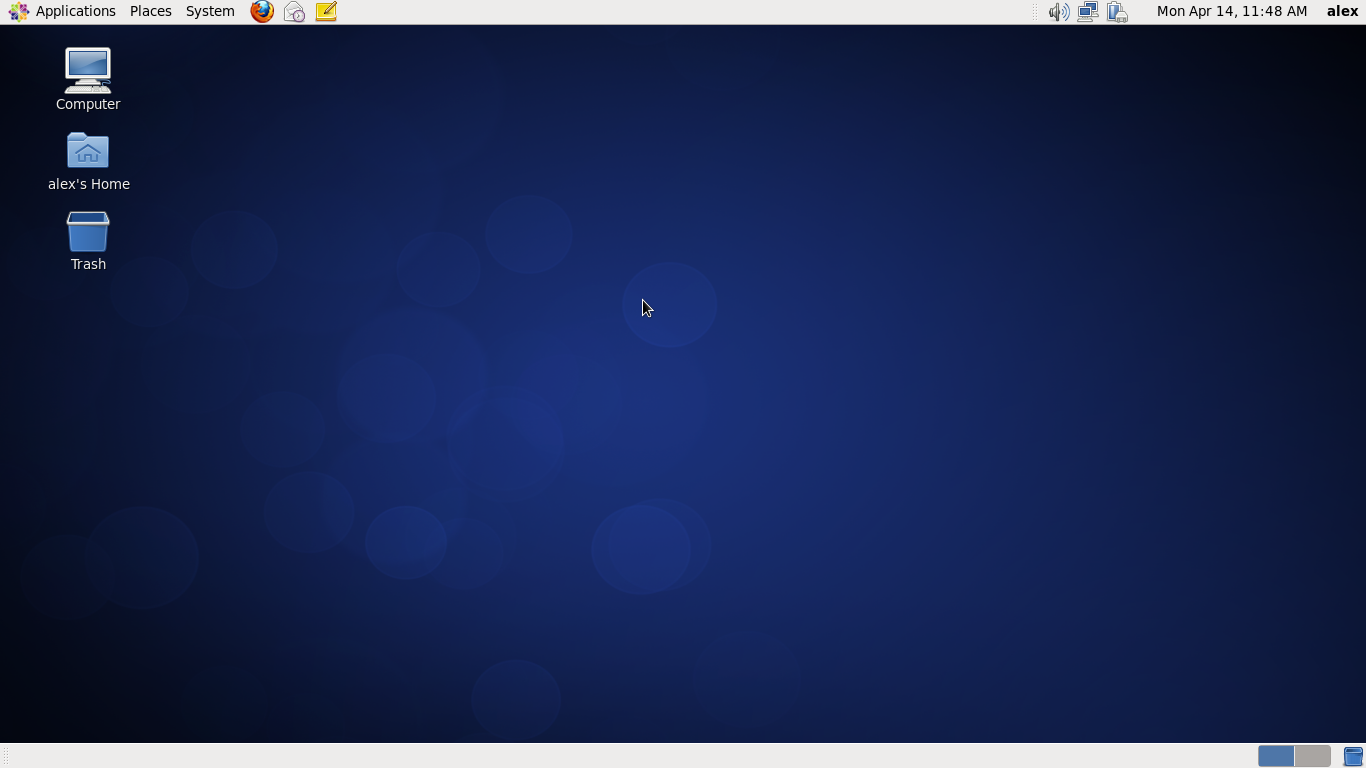
\includegraphics[scale=.24]{Immagini/UI_01.png}
 \label{fig:Gnome Desktop 2.28.2}
 \caption{Screenshot di GNOME Desktop 2.28.2 su CentOS 6.5}
\end{figure}

All'interno dell'interfaccia sono riconoscibili 3 elementi principali

\begin{itemize}
 \item panel
 \item applet
 \item workspace
\end{itemize}

\subsubsection{Panel}
Sono quelle barre, solitamente di colore grigio, presenti agli estremi dello spazio desktop. La dimensione ed il numero di questi pannelli è personalizzabile, così come il colore ed il contenuto. Nella configurazione in esempio troviamo un pannello sul bordo superiore ed inferiore del desktop. L'uso tipo è quello di contenere le applet o applicazioni speciali.
\subsubsection{Applet}
Normalmente sono visualizzabili come icone disposte sopra i vari panel. La loro funzione è variabile, e può fungere da launcher di applicazioni, così come essere un modulo di controllo per un servizio di sistema (es nm-applet di NetworkManager) o dei controlli del desktop (es. Workspace switcher)
\begin{figure}[!ht]
\centering
 
\includegraphics{Immagini/UI_Panel1.png}
 \label{fig:Panel Gnome}
 \caption{Alcune applet sulla pozione di un panel}
\end{figure}


\subsubsection{Workspace}
Si tratta dell'area di lavoro, all'interno delle quali, il gestore delle finestre posiziona le applicazioni che vengono aperte. All'interno è possibile trovare anche icone realtive ad alcuni percorsi di sistema e launcher di singole applicazioni. Differentemente da numerosi prodotti simili, Gnome offre Workspace multipli, dove è possibile collocare finestre differenti per ognun workspace. Lo switch tra i vari Workspace è ottenuto tramite la combinazione di tasti

\begin{itemize}
 \item \keys{CTRL + ALT + \arrowkeyleft }: Sposta sul workspace a sinistra
 \item \keys{CTRL + ALT + \arrowkeyright}: Sposta sul workspace a destra
\end{itemize}



%\begin{verbatim}
% [CTRL] + [ALT] + [LeftArrow]
%\end{verbatim}
%\begin{verbatim}
% [CTRL] + [ALT] + [RightArrow]
%\end{verbatim}

Esiste inolte una applet che visualizza i workspace e consente di eseguire lo switch tra di essi, che prende il nome di Workspace Switcher.

\begin{figure}[!ht]
\centering
 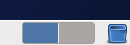
\includegraphics{Immagini/UI_WS_Switch1.png}
 \label{fig:Workspace Switcher}
 \caption{Workspace Switcher}
\end{figure}

\subsection{Applicazioni}

\subsubsection{Nautilus}

\begin{figure}[!ht]
\centering
 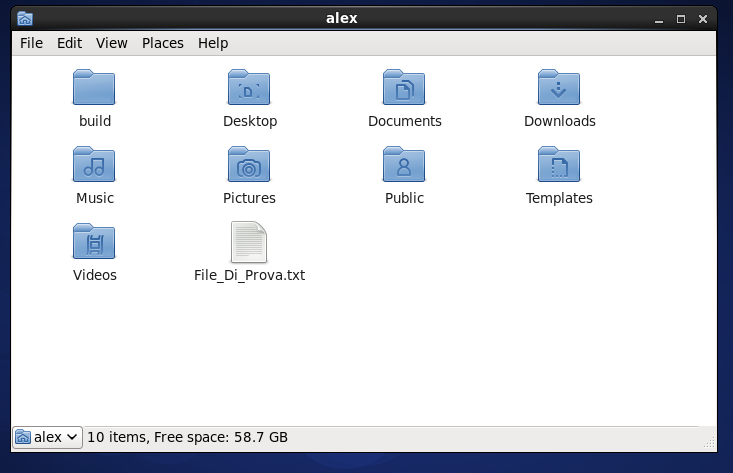
\includegraphics[scale=0.60]{Immagini/Nautilus1.png}
 \label{fig:Nautilus}
 \caption{Nautilus}
\end{figure}

\textbf{Nautilus} è un software della categoria File Manager molto potente e versatile; consente di poter consultare il contenuto delle cartelle con una intefaccia a fineste con viste configurabili. Per coloro che provengono da ambienti Microsoft\textregistered, possiamo dire che Nautilus è l'omologo Gnome del software Explorer.

Attraverso il menu \textbf{"View"} di nautilus è  infatti possibile definere la visualizzazione di file e cartelle con delle icone o con una lista organizzata. 
All'interno della lista è inoltre selezionare un criterio secondo il quale ordinare i file per ordine crescente e decrescente (es Data, Dimensione, Tipo, Nome). Inolte, con l'opzione \textbf{"Show Hidden Files"} si possono visualizzare i file marcati come "nascosti"; si tratta di file e cartelle il cui nomefile comincia con il carattere ".", ciò per impedirne la visualizzazione a meno che non sia espressamente richiesta. 

Nautilus consente di visualizzare percorsi locali (dischi interni, media rimuovibili e simili) e di percorsi remoti; attraverso la funzione \textbf{"Connect to Server"} è possibile collegarsi a macchine remote e sfruttare i file remoti come se fossero locali. I protocolli supportati sono:

\begin{itemize}
 \item Public FTP
 \item FTP Classic
 \item SSH (sftp)
 \item Windows Share (SAMBA, CIFS)
 \item NFS
 \item WebDAV
\end{itemize}

\begin{figure}[!ht]
 \centering
 \begin{subfigure}{0.4\textwidth}
  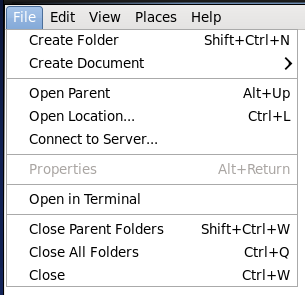
\includegraphics[scale=0.5]{Immagini/Nautilus_File2.png}
  \label{fig:Nautilus_File}
 \end{subfigure}
 \begin{subfigure}{0.4\textwidth}
  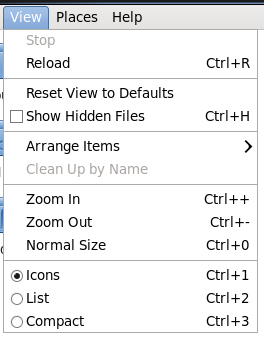
\includegraphics[scale=0.5]{Immagini/Nautilus_View2.png}
  \label{fig:Nautilus_View}
 \end{subfigure}
 \caption{Menù di Nautilus}
\end{figure}




\subsubsection{gedit text editor}

\begin{figure}[!ht]
 \centering
 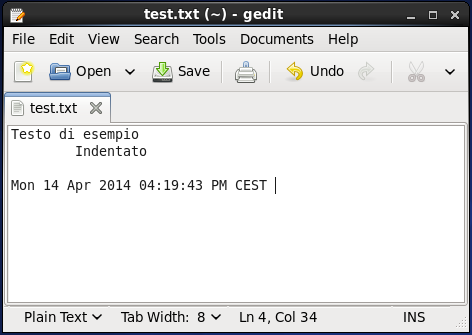
\includegraphics[scale=0.6]{Immagini/gedit1.png}
 \label{fig:gedit}
 \caption{gedit text editor}
\end{figure}


L'editor di testi \textbf{"gedit"}, è una applicazione atta alla lettura e modifica di file di testo semplici. A differenza del ben più noto omologo in ambiente Microsoft\textregistered (notepad), gedit dispone già di alcune funzioni avanzate. Ad esempio, dispone della funziona nota come \textit{"highlighting"} del codice per un gran numero di linguaggi di programmazione.

Gedit è reperibile nel menù alla voce \menu{Application > Accessories > gedit Text Editor}

\subsection{Guida in linea}

\begin{figure}[!ht]
  \centering
  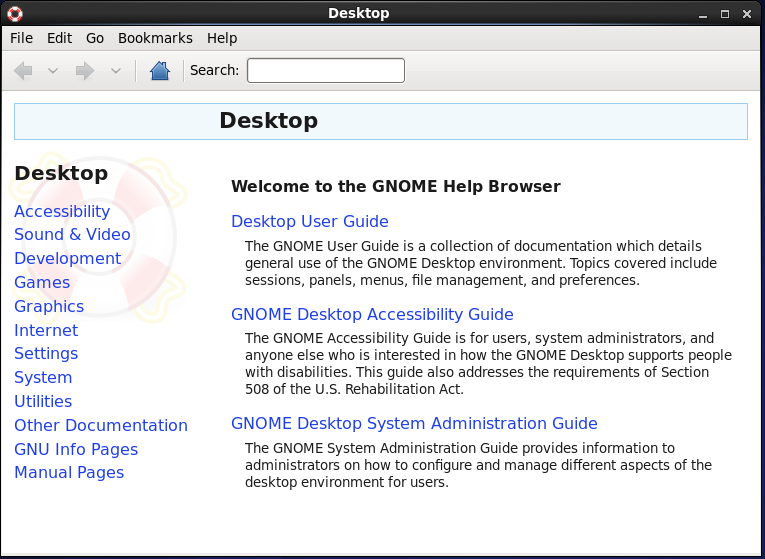
\includegraphics[scale=0.54]{Immagini/gnome_help1.png}
  \label{fig:gnome_help}
  \caption{Gnome Help}
\end{figure}

Dall'interfaccia principale di Gnome, premendo il tasto \textbf{[F1]} è possibile accedere alla guida in linea (oppure andando sul menù, selezionando la voce \menu{System > Help}. La guida è suddivisa in tre sezioni principali

% \textbf{System} $\rightarrow$ \textbf{Help})
\begin{itemize}
 \item Desktop User Guide
 \subitem Guida all'uso delle applicazioni utente, e dell'intefaccia.
 \item Accessibility Guide
 \subitem Guida per utenti ed amministratori interessati a scoprire come Gnone supporti le persone disabili nell'uso del sistema. 
 \item Administration Guide
 \subitem Guida agli strumenti di amministazione del sistema
\end{itemize}

Nel menù a sinistra è inoltre possibile consultare la guida suddivisa con il medesimo criterio di presentazione del menu delle applicazioni. 


\newpage

\section{Tool di amministrazione grafica}

\subsection{Date \& Time}

\begin{figure}[!ht]
 \centering
 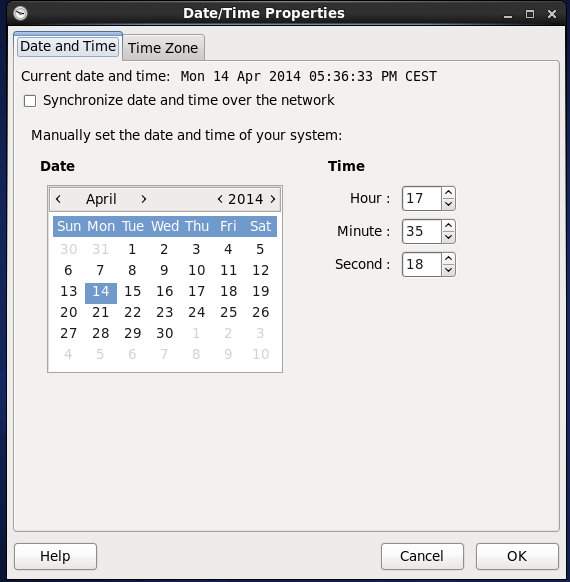
\includegraphics[scale=0.5]{Immagini/sys_conf_date1.png}
 \label{fig:System Config Date}
 \caption{system-config-date}
\end{figure}


L'utility di amministrazione ``Date \& Time'' visibile nel menu alla voce \menu{System > Administration > Date \& Time}, oppure richiamando direttamente l'applicazione \textit{system-config-date} permette la gestione di data ed ora, fuso orario e localizzazione geografica, consente di poter configurare il sistema alla interrogazione periodica di un server NTP in rete. 

Per l'uso di questa utility sono necessari i permessi di amministrazione.

%\textbf{System} $\rightarrow$ \textbf{Administration} $\rightarrow$ \textbf{Date \& Time})
\subsection{Printing}

\begin{figure}[!ht]
 \centering
 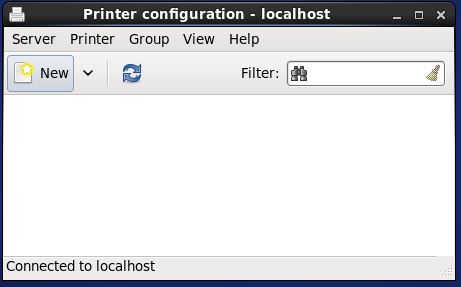
\includegraphics[scale=0.6]{Immagini/sys_conf_printing.png}
 \label{fig:System Config Printer}
 \caption{system-config-printer}
\end{figure}

L'utility di amministrazione ``Printing'', visibile nel menu alla voce \menu{System > Administration > Printig} oppure richiamando direttamente l'applicazione \textit{system-config-printer}, consente la configurazione delle stampanti di sistema, siano esse locali o remote. 

Per l'uso di questa utility sono necessari i permessi di amministrazione.

\subsection{User \& Groups}

\begin{figure}[!ht]
 \centering
 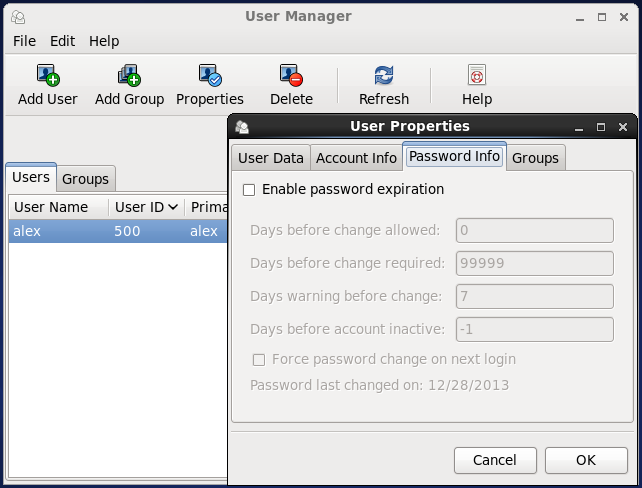
\includegraphics[scale=0.5]{Immagini/sys_conf_user1.png}
 \label{fig:System Config user}
 \caption{system-config-users}
\end{figure}




L'utility di amministazione ``User \& Groups'', visibile nel menù alla voce \menu{System > Administration > User \& Groups} oppure richiamando direttamente l'applicazione \textit{system-config-users}, consente la gestione e l'amministazione degli utenti del sistema, permettendo di poter lavorare contemporaneamente sulle informazione utente e su quelle di autenticazione. Ad esempio:

\begin{itemize}
 \item Creazione e rimozione utenti
 \item Creazione e rimozione gruppi
 \item Cambio password utenti
 \item Gestione gruppi secondari
 \item Account Expiration, Warning period e Password Expiration.
\end{itemize}


Per l'uso di questa utility sono necessari i permessi di amministrazione.
\newpage

\section{Storage}

\subsection{Hard Disk}

La conservazione dei dati informatici all'interno dei vari elaboratori elettronici avviene con tecnologie e sistemi assai diversificati tra di loro. Questi dispositivi, che prendono il nome di ``Storage Devices'' sono spessi caratterizzati da numerose differenze sul piano fisico (Dischi magnetici, Nand, Flash, supporti ottici, nastri magnetici etc..) e sulla localizzazione (storage locali o remoti). 

Lo storage device considerato più comune rimane il supporto noto come Hard Disk (HD); si tratta di uno o più piatti metallici, ricoperti da un sottile film di materiale ferromagnetico. Le differenze elettromagnetiche rappresentano le informazioni coservate sotto forma di bit. 
L'organizzazione dei dati sui dischi è generalmente basata sul modello \textit{``Cylinder/Head/Sector''} o CHS (Cilindro/Testina/Settore).

\begin{itemize}
 \item Piatto
  \subitem Un HD è composto da più dischi paralleli; ogni superficie del disco corrisponde ad un piatto.
 \item Settore
  \subitem Un piatto è suddiviso in settori circolari; corrispondo a spicchi radiali sul piatto.
 \item Traccia
  \subitem Un piatto è suddiviso in porzioni ad anello concentriche
 \item Testina
  \subitem Su ogni piatto lavora una testina di lettura/scrittura; tutte le testine sono solidali tra loro.
 \item Cilindro
  \subitem Indica lo spazio descritto da tracce equidistanti dal centro su tutti i piatti del HD.
\end{itemize}

Ad ogni modo, nonostante gli hard disk siano strutturalmente complessi, il sistema operativo offre un notevole livello di astrazione che consente di poter sfruttare lo spazio di immagazzinamento come una area contigua ed organizzata secondo schemi di partizionamento. Lo schema di partizionamento preso in esame è quello noto come \textbf{``MSDOS''}.

\begin{figure}[!ht]
 \centering
 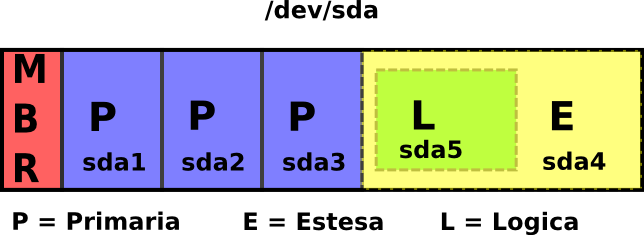
\includegraphics[scale=0.4]{Immagini/disk_scheme.png}
 \label{fig:DiskScheme}
 \caption{Schema Partizionamento}
\end{figure}

\subsubsection{M.aster B.oot R.ecord}

Il Master Boot Record (MBR) è quel settore del disco che contiene i primi 512 Byte del disco, noto anche come settore di avvio.  Al suo interno è suddiviso in 

\begin{itemize}
 \item 446 Byte: MBP Master Boot Program (stage1, lba48 pointer)
 \item 64 Byte: MBT Master Boot Table
 \item 2 Byte: Magic Number (AA 55)
\end{itemize}


Per quanto questo schema sia ampliamente utilizzato, mantiene anlcuni limiti legati ad un design datato rispetto all'evoluzione tecnica dei dispositivi di storage. 
Uno dei limiti fondamentali è legato al numero di partizioni primarie (4 al massimo); questa limitazione è in parte superata con l'adozione di partizione estese alle interno delle quali sono definibili 11 partizioni logiche. 


\subsubsection{Partizioni}

Lo spazio disponibile sul disco è suddivisibile in partizioni. Le partizioni, se pur caratterizzate per tipologie, rappresentano esclusivamente dei contenitori all'interno dei quali vengono creati dei filesystem. 
In questa fase è opportuno aver ben presente la differenza tra partizione, che è una suddivisione del dispositivo di storage, e filesystem che invece è una struttura dati atta ad organizzare i file all'interno del disco.

Nei sistemi Linux vengono utilizzati 3 tipi distinti di partizioni 

\begin{itemize}
 \item Linux (0x83): Utilizzata per i filesystem ext2/ext3/ext4 
 \item Linux swap 0x82: Utilizzata per le partizioni di swap
 \item Linux LVM 0x8e: Utilizzata per creare dei Physical Volume LVM
\end{itemize}

Una delle regole ``non scritte'' del mondo GNU/Linux è che \textit{``everything is a file''} (tutto è un file), nel senso che tutto (o quasi) all'interno del sistema, attraverso opportuni strumenti di astrazione hardware, è visibile sotto forma di file. 
Non fanno eccezioni i vari dispostivi di storage (sd), che sono solitamente allocati all'interno della cartella \textbf{/dev}; ad esempio quello che sara visto come primo disco, sara indicato con \textbf{sda} il secondo \textbf{sdb} il terzo \textbf{sdc} e cosi via.
Meccanismo analogo vale per le partizioni all'interno del disco; la prima partizione prenderà il nome di \textbf{sda1}, la seconda \textbf{sda2} e così a seguire. 
Questo meccanismo, non univoco benchè assai intuitivo, offre un primo modo di identificare dischi e partizioni per eseguire le operazioni basilari.

\subsubsection{Filesystem}

Il filesystem è la struttura dati con cui sono organizzati i dati all'interno del dispositivo di storage. Tale organizzazione varia molto sulla base del sistema operativo utilizzato; ad esempio le versioni passate dei sistemi operativi Microsoft\textregistered utilizzano una struttura nota come \textit{``Tabella di allocazione File''} (\textbf{FAT}: File Allocation Table), mentre i sistemi Unix e derivati si basano su una sistema basato su \textbf{inode}. 

I filesystem trattati in questo testo sono:

\begin{itemize}
 \item ext2: Second Extended Filesystem
 \subitem: Filesystem basato su inode, semplice e prestazionale sulle piccole dimensioni 
 \item ext4: Fourth Extended Filesystem
 \subitem Evoluzione di ext3, 48bit, journaled, default dei sistemi GNU/Linux odierni.
 \item FAT: File Allocation Table
 \subitem Filesystem molto semplice di derivazione Microsoft\textregistered, limitato
 \item xfs: XFS, Silicon Graphics
 \subitem Filesystem 64bit, B-tree+, ideale per grandi volumi
 \item glusterfs
 \subitem Filesystem ideato per lavorare su sistemi cluster
\end{itemize}

A seguire alcune caratteristiche notevoli dei filesystem presi in considerazione

\begin{center}
\begin{tabular}{|l|ccr|}
\hline
 & Max. File & Max. Vol.  & FilenameChar \\
\hline
ext2 (1K) & 16 GiB & 2 TiB & 255 \\
ext2 (8K) & 2 TiB & 32 TiB & 255 \\
ext4 & 16 TiB & 1 EiB & 255 \\
xfs & 8 EiB & 16 EiB & *\\
FAT32 & 4GiB & 124/2048 GiB & 255 \\
\hline
\end{tabular}
\end{center}



\subsubsection{Mount Point}

A differenza dei sistemi operativi Microsoft\textregistered, dove di solito le partizioni vengono indicate con il nome di unita logiche (es. C:, D: etc..), per utilizzare i vari filesystem (locali e remoti) è necessario ``montarli'' su un percorso all'interno dell'abero delle cartelle. 
Al momento dell'avvio del sistema viene impostata la cartella radice (root directory indicata con \textbf{``/''}, da non confondere con la cartella dell'utente root che si trova su \textbf{``/root''}.
Tutti i filesystem montati successivamente saranno visibili in sotto directory della cartella radice specificate al momento del mount. Alcune cartelle sono di solito dedicate a questa funzione come la \textbf{/mnt} o per i media removibili su \textbf{/media}. Ciò vale anche per supporti esterni quali CD/DVD, USB Mass Storage e filesystem di rete (es. NFS e CIFS).


\subsubsection{Disk Utility}

\begin{figure}[!ht]
 \centering
 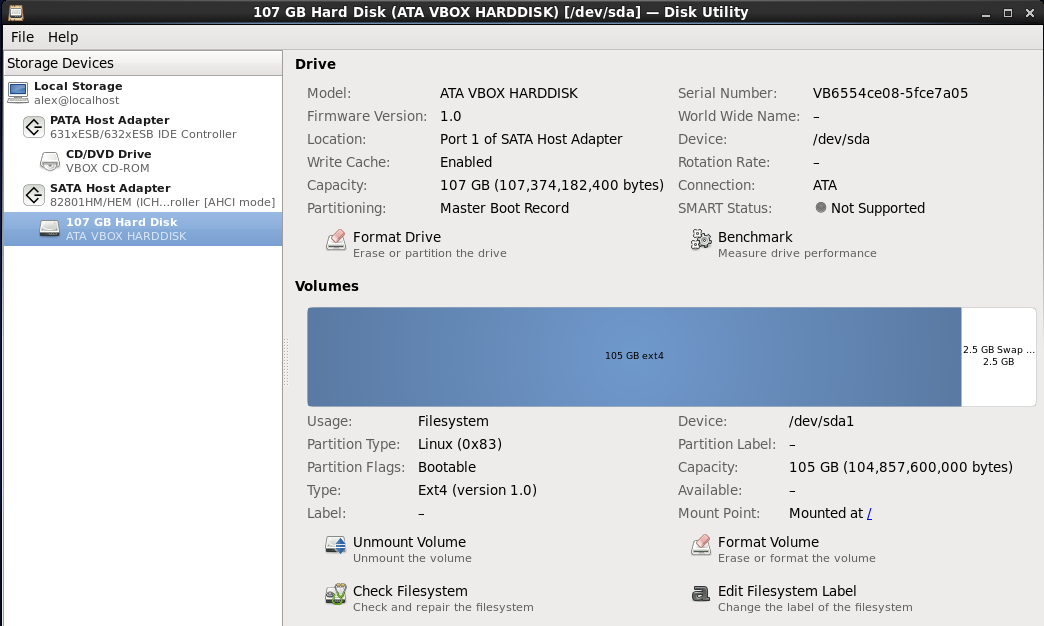
\includegraphics[scale=0.4]{Immagini/Disk_Utility1.png}
 \label{fig:DiskUtility}
 \caption{Disk Utility}
\end{figure}

Per la gestione delle partizioni, all'interno del sistema è presente la \textbf{``Disk Utility''}, uno strumento dalla grafica intuitiva, che consente di identificate il disco interessato, creare, rimuovere modificare partizioni, formattarle e stabilire un punto di mount. 

\subsubsection{Comandi per partizioni e filesystem}

TODO

\subsection{LVM}

\begin{figure}[!ht]
  \centering
  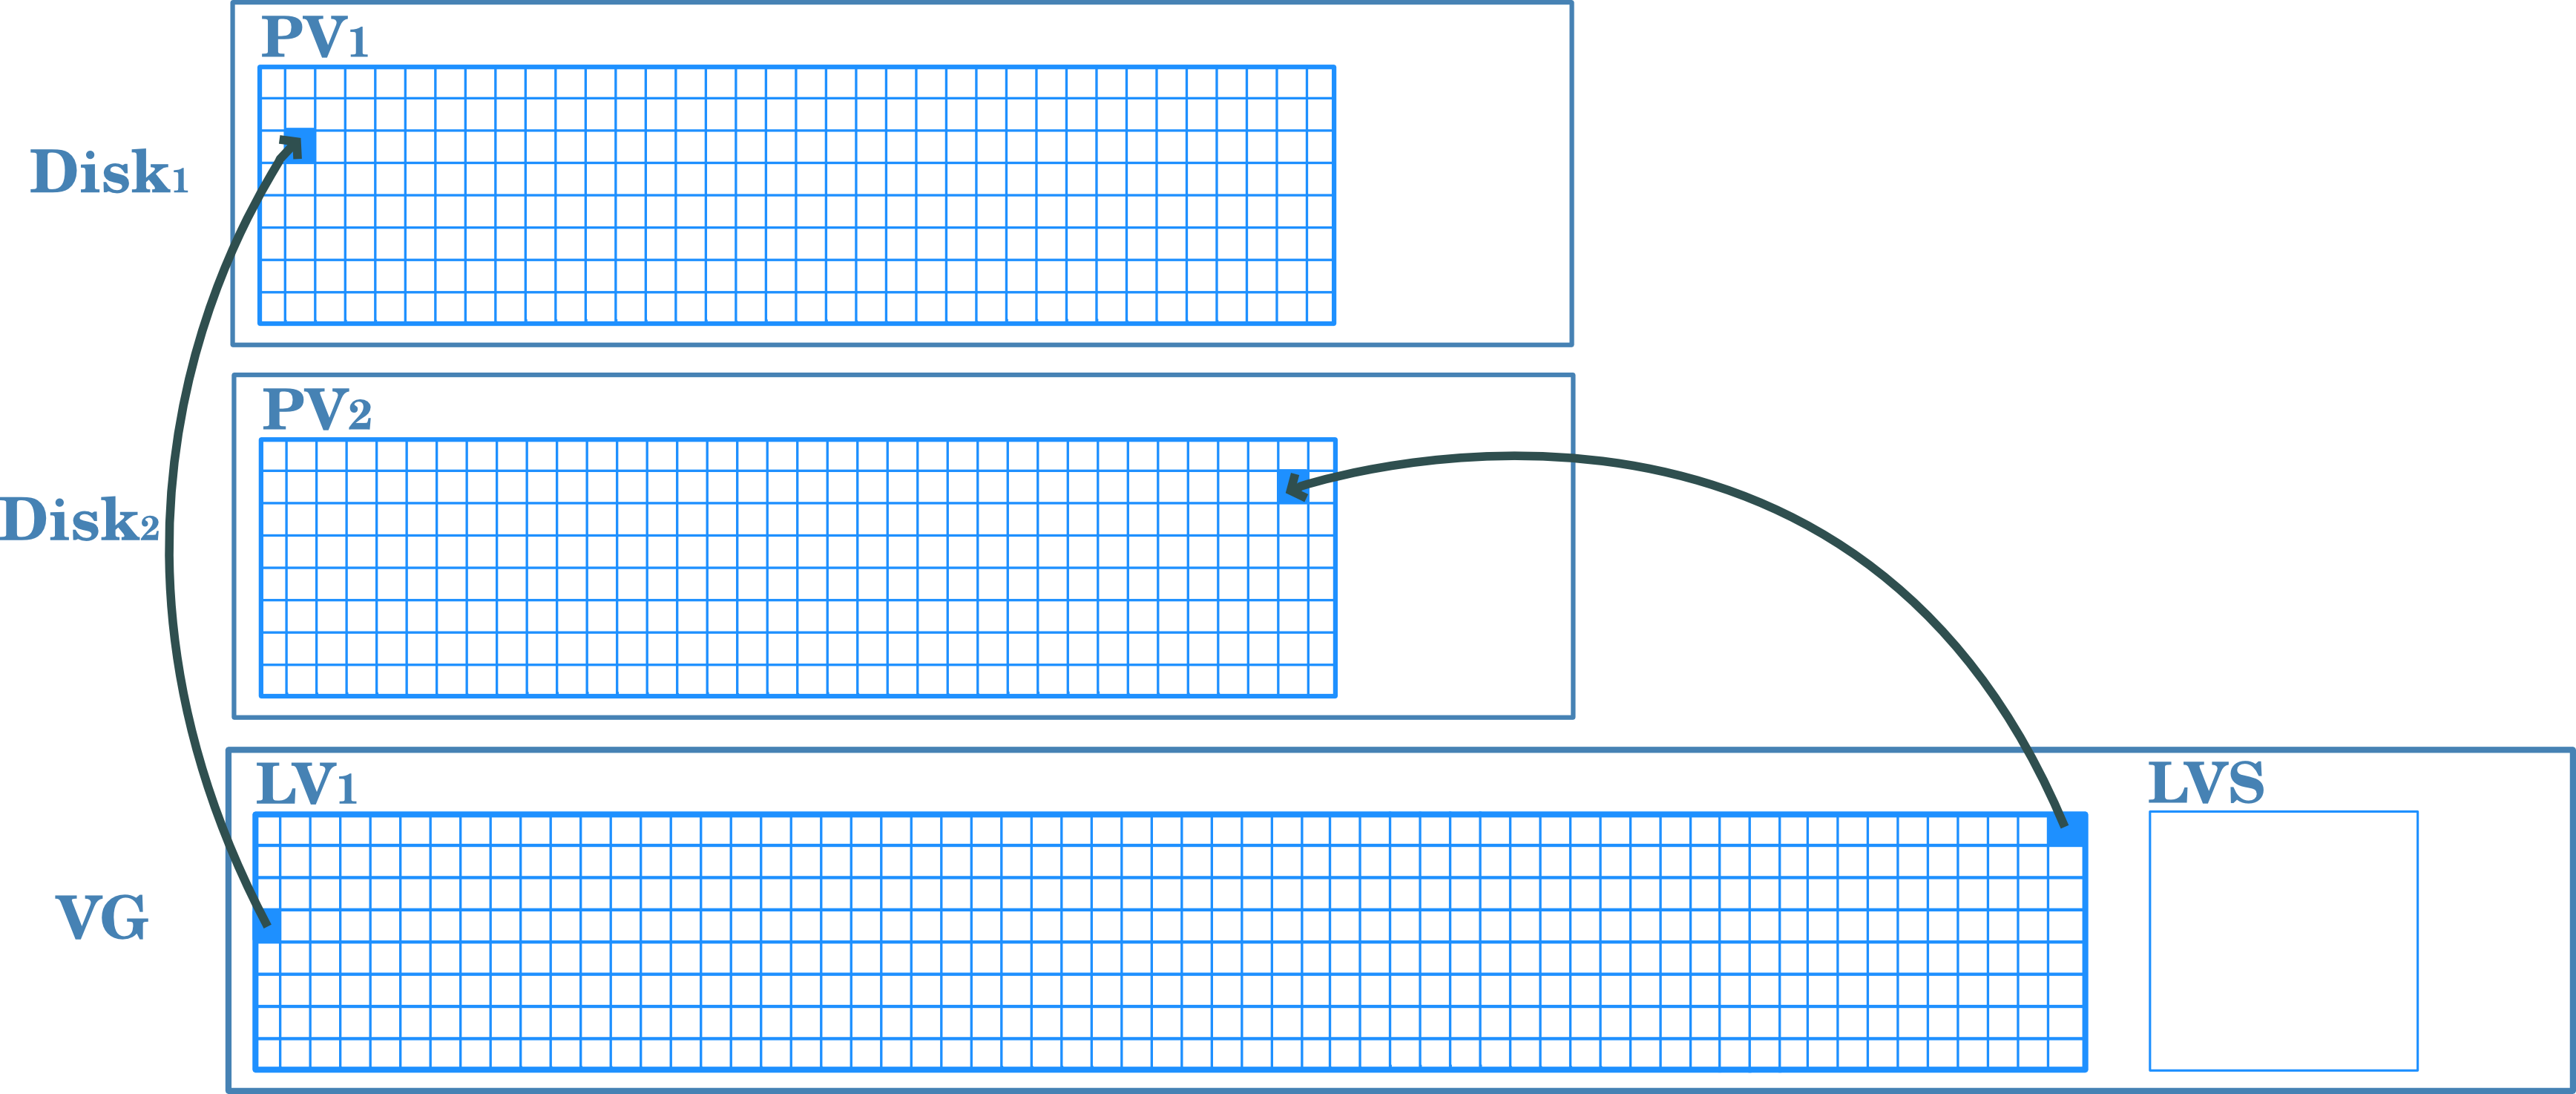
\includegraphics[scale=0.4]{Immagini/partitions.png}
  \label{fig:LVM_scheme}
  \caption{Volume Group composto da due Physcal Volume}
\end{figure}



Il Logical Volume Manager è uno stato software che crea un livello di astrazione più alto sopra dischi e partizioni, tale da superare i limiti imposti dal livello fisico, offrendo continuità tra dischi differenti, flessibilità ed affidabilità.

All'interno del LVM è utile identificare gli elementi che lo compongono

\begin{itemize}
 \item PP: Physical Partition
 \subitem Partizione fisica di tipo Linux LVM (0x83).
 \item PV: Physical Volume
 \subitem I physcal volume sono le PP inizializzate che andranno a comporre il volume group.
 \item VG: Volume Group
 \subitem L'astrazione a livello software che mostra tutti i physical volume con un unico dispositivo di storage. Lo spazio al suo interno è diviso in \textbf{``extens''}, che devono essere di dimensione omogenea tra i vari PV. 
 \item LV: Logical Volume
 \subitem Rappresentano le ``partizioni'' all'interno del Volume Group. Sono estensibili e formattabili con i filesystem ext4. 
 \item PE: Physical Extens
 \subitem Sono i blocchi funzionali con cui i VG mappano lo spazio di allocazione sui vari PV. Le dimesione dei PE è variabile in base al tipo di prestazioni che si vogliono enfatizzare.  
 \item LE: Logical Extens
 \subitem Sono i blocchi funzionali di mappatura ta il LV ed il VG. A meno che i PV non siano configurati in ``mirror'', ad ogni LE, corrisponde un PE. 
\end{itemize}

L'utilizzo di LVM consente facilmente di superare i limiti legati agli schemi di partizionamenti tradizionali in termini di numero di partizioni, ma anche di dimensione allocabile (il VG, nella configurazione normale, è uguale alla somma dei PV che lo compongono, a meno di configurazione ``mirror''). 
Inoltre, il superiore livello di astrazione consente all'amministratore di variare la dimensione del LV, modificando il filesystem in esso contenuto. 
Tale operazione, nel caso si tratti di una \textbf{estensione} è generalmente considerata sicura, ed è effettuabile anche a caldo (ovvero quando il filesystem che insiste su LV risulta montato). Ciò non è altrettanto vero parlando di \textbf{riduzione}, dove per varie ragioni tecniche, è raccomandabile eseguire un backup dei dati contenuti, e non è possibile effetturare questa operazione a caldo. 
Un'altra potrnzialità ovverta da LVM, è la possibilità di creare degli Snapshot (LVS); uno snapshot è una sorta di immagine virtuale di un LV in utilizzo, realizzato dedicando una area del volume group apposita, dove vengono salvate solo le versioni originali dei file modificati.
Qualora le modifiche al LV risulteranno valide è possibile scartare lo snapshot, in caso contrario è possibile eseguire una operazione di merge che riporta alla configurazione ``fotografata'' al momento della creazione dello snapshot.

\subsubsection{Logical Volume Management}
%\textbf{System} $\rightarrow$ \textbf{Administration} $\rightarrow$ \textbf{LVM}

Questa applicazione, visibile nel menu sotto \menu{System > Administration > LVM} (nome applicazione: \textit{system-config-lvm}) consente di creare, gestire e modificare i Physical Volume, i Volume Group ed i Logical Volume.

\begin{figure}[!ht]
 \centering
 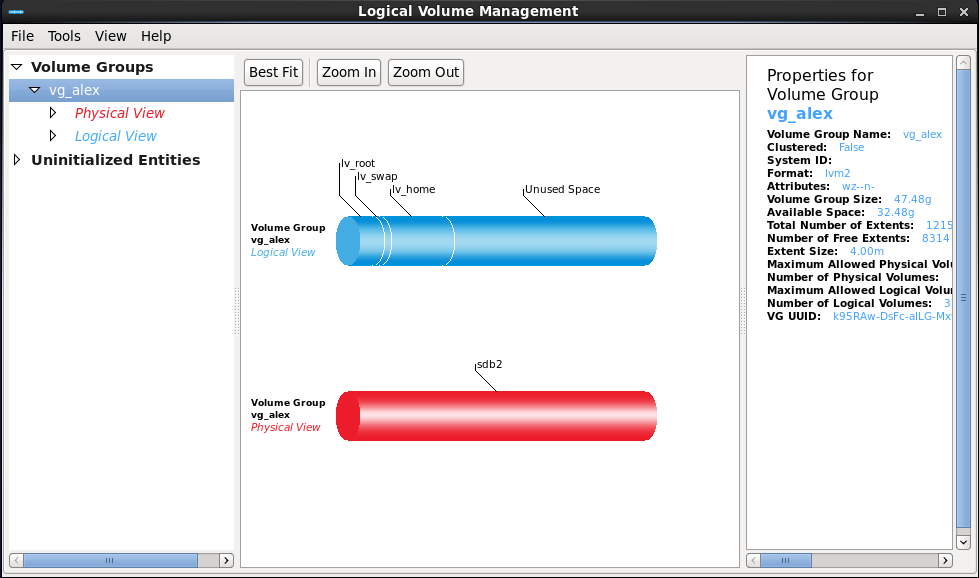
\includegraphics[scale=0.4]{Immagini/LVM_utility.png}
 \label{fig:LVM Utility}
 \caption{LVM Utility}
\end{figure}


\subsubsection{Comandi da terminale per LVM}

TODO


\newpage

\section{La Shell}

\subsection{Il terminale}

Con ``terminale'' si indica un particolare tipo di attrezzatura hardware atta alla ricezione ed invio di input/output. All'epoca dei primi computer, si trattava di unita composte da tastiera e monitor (dispositivi a caratteri) prive di una CPU propria (per questo erano anche noti come ``terminali stupidi), collegate attraverso porte seriali all'elaboratore principale.
Nonostante ad oggi questo approccio sia superato, ancora oggi, nei sistemi ispirati fortemente a Unix è rimasta la modalità di interfacciamento attraverso terminali. In Linux, pur non essendo realmente hardware (si parla di \textbf{Virtual Terminal}), sono ancora trattati come tali, e sono visibili nella cartella delle periferiche (\textbf{/dev}) sotto forma di \textbf{tty\textit{X}} (dove il valore di \textbf{\textit{X}} è un numero progressivo).

A livelli di ``astrazione'' più alta (es. nelle interfacce grafiche o con ssh) si utilizzano un altro tipo di terminali, definiti \textbf{``Pseudo Terminal''} (es pts/0). Nonostante vi siano notevoli differenze sul piano dell'implementazione software, non sono rilevanti ai fini dell'utilizzo comune. 
Di particolare importanza è invece evitare la confusione tra la dicitura ``terminale'' e quello di ``shell'', anche se spesso, anche in letteratura, vengono confusi. 

\subsection{La shell}

La shell è uno strumento software che permette, attraverso dei comandi, di comunicare con il Sistema Operativo. In molti casi, la shell prende anche il nome di ``Interprete dei Comandi''. 
Nella storia dei sistemi operativi Unix-ware prima, e Linux negli ultimi anni, si sono succedute diverse implementazioni di shell, differenti per caratteristiche tecniche e modalità d'uso. 
Per funzionare, una shell sia appogia ad un terminale, sia esso fisico (es delle porte seriali), virtuale (tty1,tty2... etc) o uno \textit{pseudo terminal} (es. gnome-terminal).
Ripercorrendo la storia delle shell, tra le prime a venire fuori ci sono state la \textbf{sh} (Bourne Shell, prende il nome da Stephen Bourne, suo ideatore) e la \textbf{csh} (C-Shell, prende il nome dal fatto di avre una sintassi prossima a quella del linguaggio di programmazione C). 
Ad oggi, non si usano più quelle versioni, ma delle versioni ad esse ispirate, come ad esempio la \textbf{tcsh} (presente in molti sistemi ``BSD-like'') la \textbf{ksh} (Korn Shell, di ideazione più recente, molto usata nei sistemi Oracle\textregistered, e la \textbf{bash} (Bourne Again Shell) utilizzata come shell predefinita nella maggior parte dei sistemi GNU/Linux, sarà usata come shell di riferimento in questo testo. 

Tra le particolarità di queste shell, oltre ad alcune differenze funzionali, c'è il fatto che ognuna di esse dispone di un proprio linguaggio di scriptig

\subsection{Bash}

Bash è una shell completa, dotata di un potente linguaggio di scripting, ampiamente utilizzato in tutto il mondo GNU/Linux (e non solo). Fornisce, oltre all'accesso a tutti i comandi del sistema, una serie di strutture iterative e di controllo di flusso, garantisce l'uso di variabili d'ambiente (non tipizzate), autocompletamento dei comandi e degli argomenti (ma non delle opzioni) e, tra le altre cose, delle combinazioni di tasti per il controllo delle attività. 

La shell offre da subito una serie di informazioni utili, immediatamente dopo il login
\begin{verbatim}
 [user@hostname ~]$
\end{verbatim}
Esaminando i campi uno ad uno
\begin{itemize}
 \item \textbf{user}: l'utente con cui si è collegati
 \item \textbf{hostname}: il nome della macchina a cui si è collegati
 \item \textasciitilde: La cartella in cui ci si trova. La "\textasciitilde" indica la propria cartella HOME
 \item \$: Il tipo di utenza. Con \$ si tratta di utenze "normali", con \# di utenze di amministrazione
\end{itemize}

Nonostante alcune variazioni sul tema, variabili da comando a comando, solitamente la sitassi lanciare un comando dalla shell è del tipo:

\begin{verbatim}
 [user@hostname.domain ~]$ commando -o --opzione-lunga argomento1 
\end{verbatim}

Scomponendo l'esempio otteniamo

\begin{itemize}
 \item \textbf{comando}: il comando che si vuole lanciare
 \item \textbf{-o}: Si tratta di una opzione in formato corto, composta da un "-" ed un singolo valore alfanumerico. Quasi tutti i comandi offrono opzioni di questo tipo. In presenza di più di questo tipo di opzioni, esse possono essere sommate in una stringa (es. -p -r -o possono essere scritte con -pro).
 \item \textbf{--opzione-lunga}: Anche questo tipo di opzioni sono comuni. Anche se generalmente molte di queste opzioni hanno un opportuno omologo in formato corto, vengono spesso utilizzate per facilitare la lettura di script o l'approccio mnemonico ai comandi. 
 \item \textbf{argomento1}: In generale, è il contenuto su cui lavorerà il comando lanciato. Può fare riferimento ad un elevato numero di cose (file, cartelle, device, indirizzi web, riferimenti in memoria etc, etc...)
\end{itemize}

Come già anticipato, ci sono alcune sequenze di controllo che permettono, digitando le opportune combinazioni di tasti, di mandare degli specifici segnali, o eseguire alcune operazioni sulla shell.

\begin{itemize}
 \item \keys{CTRL + c} - SIGINT (2): Interruzione del processo da tastiera
 \item \keys{CTRL + z} - SIGTSTP (18,20,24): Ferma il processo e lo lascia in stato ``stopped''
 \item \keys{CTRL + r} - RESEARCH: Consente la ricerca nella history dei comandi
 \item \keys{CTRL + d} - SIGQUIT (3): Invia il segnale di uscita dalla tastiera, ma è utilizzato anche con funzione di ``logout'' e di EOF
 \item \keys{CTRL + a} - HOME: Riporta il cursore alla posizione iniziale
 \item \keys{CTRL + b} - END: Porta il cursore in fondo alla riga
\end{itemize}


%\subsubsection{}






\newpage

\section{Processi}


In letteratura ci si riferisce al termine ``processo'' come ad una istanza di un programma eseguito in modo sequenziale (che può essere o meno multithread in base al sistema operativo) su un processore. Tale concetto non è da confondersi con il concetto di thread, anche se in alcuni casi può coincidere con il processo.

In generale, si considerano i vari processi come entità concorrenti all'uso delle risorse del sistema (CPU, ram, I/O, etc..). Il sistema operativo gestisce l'accesso alle risorse, ed offre gli strumenti per controllare i processi, attraverso l'uso di ``segnali''. 

Tutti i processi vengono identificati all'interno del sistema attraverso un PID (Process IDentifier o identificativo di processo), ovvero un numero progressivo che solitamente va da 1 a 32768 (\directory{/proc/sys/kernel/pid\_max}). 

Il numero PID assunto da un processo non è predicibile, ma è noto che i primi PID sono relativi a processi di sistema, mentre il processo con PID 1 è sempre il processo di \textbf{init}.

All'infuori di \textbf{init}, tutti i processi presenti nel sistema, sono in un rapporto parentale con altri; ogni processo, nel momento in ``lancia'' (fork) un altro processo, diventerà il processo ``padre'' del processo lanciato. Contestualmente, il processo lanciato diventerà il processo ``figlio'' del processo chiamante.

La struttura padre/figlio dei processi offre una ottima struttura gerarchica di controllo dei processi. 

Alcune definizioni

\begin{itemize}
 \item Processo padre: processo che esegue una chiamata di tipo \textit{``fork()''} (seguita spesso da una \textit{exec()})
 \item Processo figlio: processo creato dalle chiamate del processo figlio
 \item Processo orfano: Processo che ha perso il processo padre, e viene ``adottato'' da init (re-parenting)
 \item Processo zombie (defunct): processo figlio sul quale il processo padre non ha eseguito la chiamata di wait() per leggerne il valore di ritorno. Per questo motivo il PID risulta ancora nella lista processi.  
\end{itemize}

Il sistema di comunicazione tra i processi ed il sistema è basato su notifiche asincrone definite segnali. A seguire alcuni di quelli definiti dallo standard POSIX (Portable Operating System Interface for Unix):

\begin{itemize}
 \item SIGHUP (1): Chiusura di un terminale.
 \item SIGINT (2): Interruzione da tastiera
 \item SIGQUIT (3): Segnale di uscita dalla tastiera
 \item SIGILL (4): Istruzione illegale (Illegal instruction)
 \item SIGABRT (6): Segnale di abbandono (abort)
 \item SIGFPE (8): Eccezione in virgola mobile
 \item SIGKILL (9): Termina il processo
 \item SIGSEGV (11): Riferimento in memoria non valido (segmentation fault)
 \item SIGPIPE (13): Broken Pipe
 \item SIGTERM (15): Segnale di terminazione
 \item SIGCHLD (20,17,18): Processo figlio terminato.
 \item SIGSTOP (17,19,23): Segnale di stop del processo
 \item SIGTSTP (18,20,24): Segnale di stop da tastiera
\end{itemize}


Il \textbf{SIGKILL} ed il \textbf{SIGTERM}, se pur simili, operano in modo diverso: il segnale di KILL, corrisponde ad una chiusura immediata, e non può essere ignorato. Il segnale di TERM invece consente al processo di eseguire le operazioni di uscita.  

Tutti i segnali possono essere intercettati, bloccati o ignorati, ad eccesione del segnale SIGKILL(9) e SIGSTOP(

Il comando per inviare i segnali ai vari processi è noto come \textit{kill}, e prende il nome dal segnale n. 9, erroneamente considerato il segnale di default del comando, che invece è il SIGTERM(15).

\begin{verbatim}
 $ kill -9 2345
 $ kill 2346 2349
\end{verbatim}

\subsection{Priorità}

Lo scheduler è quella parte dei sistema operativo che garantisce la concorezza alle varie risorse hardware. Per motivi di effecienza computazionale gli scheduler hanno un comportamento non predicibile, tuttavia è possibile influenzare il suo comportamento sfruttando il meccanismo della priorità.

La priorità consente di stabilire un ordine di esecuzione preferenziale, tale da garantire ai singoli processi un diverso accesso alle risorse (in particolare il processore). Nei sistemi di derivazione Unix, vale il concetto di \textbf{``niceness''}; si tratta di un valore inversamente proporzionale alla priorità. Minore è il valore di niceness, maggiore è la priorità, e viceversa. 
Alcuni valori di niceness (da -20 a -1) sono ad uso esclusivo dell'utente amministratore (root), questo per motivi di sicurezza ed efficienza del sistema operativo.  A meno di poche eccezioni, i processi partano con un valore di niceness uguale per tutti considerato come default (solitamente 0).

\begin{figure}[!ht]
 \centering
 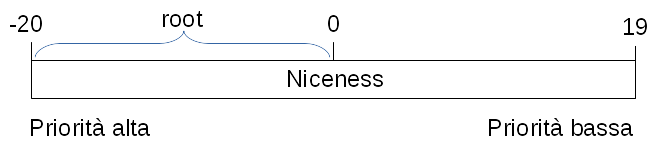
\includegraphics[scale=0.65]{Immagini/niceness.png}
 \label{fig:Niceness}
 \caption{Priorità}
\end{figure}

Due comandi tipici per impostare e reimpostare la priorità ad un processo sono rispettivamente il comando \textbf{nice} e \textbf{renice}. Ad esempio

\begin{verbatim}
 $ nice -10 /usr/bin/firefox
 $ renice -5 2345
\end{verbatim}


\subsection{System Monitor}

\begin{figure}[!ht]
 \centering
 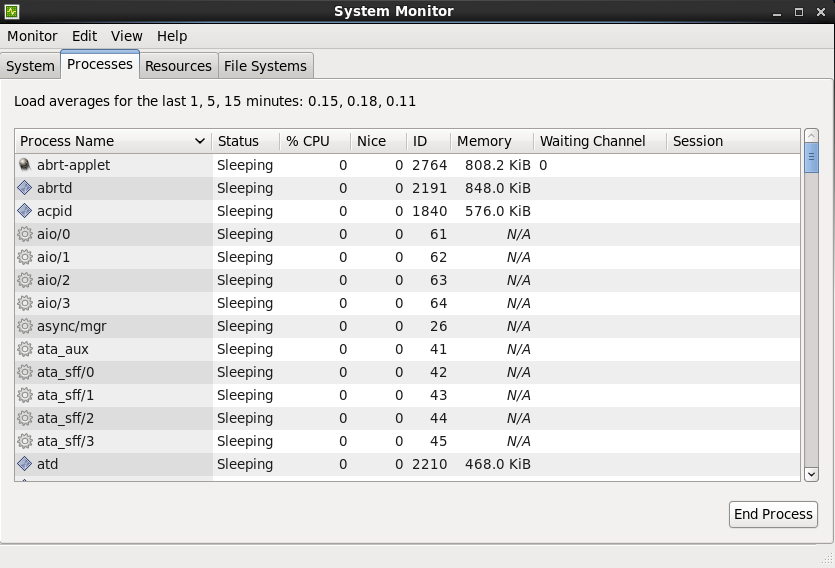
\includegraphics[scale=0.4]{Immagini/sys_mon1.png}
 \label{fig:System Monitor}
 \caption{System Monitor}
\end{figure}

System Monitor (gnome-system-monitor), presente nel menu alla voce \menu{Applications > System Tools > System Monitor}, è una pratica applicazione da UI, che consente di svolgere numerose operazioni

\begin{itemize}
 \item Visualizzare tutti i processi
 \item Visualizzare l'uso delle risorse (RAM, CPU, dischi, rete)
 \item Cambiare priorità ai processi
 \item Inviare segnali ai processi (9 e 15)
 \item Controllare le risorse sfruttate da ogni singolo processo
 \item Visualizzare l'abero gerarchico dei processi
\end{itemize}


\subsection{Gestione processi da terminale}


\subsubsection{ps}

Il comando \textbf{ps} (process status) mostra i processi presenti nel sistema. Si tratta di un comando con un numero considerevole di opzioni. Per varie ragioni mantiene la compatibilità di opzioni sia con quelle definite POSIX, e quelle BSD. Per non confondere i due tipi di opzioni, sotto Linux si possono usare le opzioni di tipo BSD, omettendo il carattere ``-''. 

Alcune opzioni POSIX:

\begin{itemize}
 \item ``-e'': Tutti i processi di tutti gli utenti
 \item ``-f'': Tutte le informazioni relative ai processi
 \item ``-l'': Formato esteso delle informazioni
 \item ``-p [lista-pid]'': Visualizza le informazioni sui processi con i pid selezionati
\end{itemize}

Alcune opzioni BSD

\begin{itemize}
 \item ``a'': Tutti i processi di tutti gli utenti
 \item ``x'': Mostra processi che non hanno un terminale controllante
 \item ``u'': Formato con informazioni su uso CPU
 \item ``p [lista-pid]'': Visualizza le informazioni sui processi con i pid selezionati
\end{itemize}

Ad esempio, i due modi più utilizzati per visualizzare tutti i processi di sistema (con output leggermente differenti) sono

\begin{verbatim}
 $ ps aux
 $ ps -ef
\end{verbatim}

Il comando \textbf{pstree} mostra tutto l'albero ``geneaologico'' dei processi attivi nel sistema. 

\subsubsection{top}

Il comando \textbf{top} offre una valida alternativa utilizzabile da shell a System Monitor. Top infatti visualizza dinamicamente le informazioni sul sistema e sui processi attivi, ordinandoli per consumo di CPU (oppure di memoria), fornendo anche la possibilità di interagire con i processi.

\begin{itemize}
 \item ``h'': Guida del programma
 \item ``k'': Invio di un segnale ad un processo (kill)
 \item ``r'': Permette di cambiare la niceness di un processo (renice).
 \item ``1'': Mostra/Nasconde le informazioni divise per singolo core
 \item ``q'': Uscita dal programma
\end{itemize}

Ad oggi esistono varianti del comando top, che, pur non essendo di default, sono installabili in un secondo momento quali \textbf{atop} e \textbf{htop}.


\newpage

\section{Gestione del Software}

\subsection{I pacchetti}

Nel mondo delle distribuzioni GNU/Linux, per l'installazione, la rimozione e l'aggiornamento del software si usano dei particolari file binari (solitamente compressi), che prendono il nome di packages (pacchetti).

Nel corso dello sviluppo delle varie distribuzioni, i vari team di sviluppo hanno scelto di differenziare molto, sia per tipologia di pacchetto (rpm, deb, tgz...) sia per gestore di pacchetti (rpm, dpkg, pkgtool...).

Di fatto, ad oggi, non esiste uno standard valido per qualsiasi distribuzione, anche se molte di queste hanno scelto RPM come soluzione. RPM (Red Hat Package Manager) è utilizzato fra le altre da Red Hat e derivate (Red Hat, Fedora, CentOS...), da SUSE (e derivate) e da Mandriva. Questo rende il pacchetto RPM tra i più diffusi in assoluto. 

L'utilizzo del medesimo pacchetto da parte di distribuzioni differenti non garantisce però che i pacchetti siano compatibili tra loro, e nemmeno l'utilizzo del medesimo front-end. In base alla distribuzione infatti, è possibile vedere dei front-end differenti.

\begin{itemize}
 \item yum: Red Hat Enterpise Linux (5.x o successive), Fedora, CentOS (5.x o successive), Yellow Dog, Oracle Linux
 \item zypper: SUSE Linux Enterpise, openSUSE
 \item urpmi: Mandriva, Mageia
 \item up2date: Red Hat Enterpise Linux (precedenti a 5.x), CentOS (precedenti a 5.x), Oracle Linux
\end{itemize}

Il nome del file di un pacchetto rpm è solitamente così composto:

\begin{verbatim}
 <nome>-<versione>-<build>-<distribuzione>-<architettura>.rpm
\end{verbatim}

\begin{itemize}
 \item Nome: Nome del software
 \item Versione: Versione di rilascio del sorgente da cui è stato ricavato il pacchetto.
 \item Build: Numero di volte che la medesima versione del sorgente è stata compilata
 \item distribuzione (opzionale): in alcuni casi si indica la distribuzione di destinazione (es ``rhel6``)
 \item architettura: Codice che rappresenta l'architettura per cui il pacchetto è stato compilato (es. x86, x86\_64, arm, powerpc etc...)
\end{itemize}

Un pacchetto RPM, oltre ad avere la parte binaria, dispone anche di un ``header'', dove sono contenute alcune informazioni importanti relative al pacchetto. 

I pacchetti RPM, al momento dell'installazione, possono essere verificati attraverso i cosidetti algoritmi di summury (MD5) o attraverso verifica di firma crittografica (GPG). Con tali meccanismi si cerca di correggere eventuali errori di download e di evitare la presenza di pacchetti la cui provenienza non sia certificata. 

\subsubsection{Dipendenze}


\begin{figure}[!ht]
 \centering
 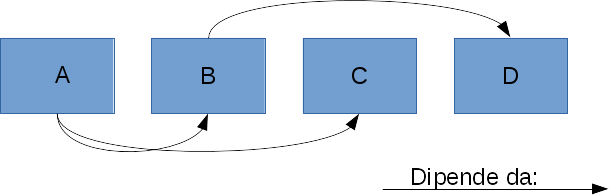
\includegraphics[scale=0.55]{Immagini/dipendenza01.png}
 \label{fig:Dipendenza}
 \caption{Relazione di dipendenza}
\end{figure}

Con i gestori di pacchetti moderni è stato introdotto il concetto di ``dipendenza''. Di fatto, buona parte del software presente in una distribuzione GNU/Linux è in dipendenza di qualche altro software. Una dipendenza è per l'appunto il software necessario ad un altro per funzionare correttamente. 
La verifica delle dipendenze al momento dell'installazione consente di controllare se è presente tutto il software necessario al pacchetto per funzionare. Inoltre, il medesimo processo applicato al momento della rimozione di un pacchetto, evita di andare a rimuovere elemnti utili ad un qualsiasi altro programma. Infine, sempre a mezzo di queste operazioni di verifica, si evita di installare pacchetti in potenziale conflitto fra di loro. 

Le informazioni sui vari pacchetti vengono conservati all'interno di un database di tipo db4 nella cartella \directory{/var/lib/rpm}

\subsection{Il tool rpm}

Il tool rpm, è il comando base da utilizzare per eseguire le varie operazioni sui pacchetti. 

Utilizzato da riga di comando la sua sintassi è

\begin{verbatim}
 # rpm <opzioni> nomepacchetto-versione-build-arch.rpm
 # rpm <opzioni> nomefile
\end{verbatim}

Alcune delle opzioni utilizzabili con rpm

\begin{itemize}
 \item \textbf{-i}: Installare il pacchetto (install)
 \item \textbf{-e}: Rimozione del pacchetto (erase)
 \item \textbf{-U}: Aggiornamento del pacchetto (upgrade)
 \item \textbf{-V}: Verifica del pacchetto installato (verify)
 \item \textbf{-q}: Informazioni sul pacchetto (query)
\end{itemize}

L'opzione ``-q'' offre altre opzioni a cui è abbinabile

\begin{itemize}
 \item \textbf{-qa}: Interroga tutti i pacchetti installati
 \item \textbf{-qf [nomefile]}: Interroga il pacchetto proprietaro del file
 \item \textbf{-qi}: Mosrta le info su un determinato pacchetto
 \item \textbf{-ql}: Mostra l'elenco dei file contenuti nel pacchetto
 \item \textbf{-qs}: Mostra lo stato dei file del pacchetto
 \item \textbf{-qc}: Mostra un elenco dei file di configurazione
\end{itemize}

\subsection{Yum}

Nonostante rpm copra un grande numero di funzioni, nel corso degli anni si sono sviluppati dei front-end per automatizzare alcune operazioni relative all'installazione e all'aggiornamento del sistema. 
Nei sistemi di stretta derivazione Red Hat si utilizza \textbf{yum} (Yellow-dog updater modified); si tratta di un programma, scritto in python che permette di installare, rimuovere, aggiornare e verificare i pacchetti. Inoltre yum, collegandosi a delle particolari locazioni (remote o locali) definite \textbf{``repository''}, scarica il software oggetto di installazione o di aggiornamento e le relative dipendenze. Tutto questo viene fatto in maniera trasparente all'utente.

La sintassi del comando yum è 
\begin{verbatim}
 # yum <opzioni> comando [argomenti]
\end{verbatim}

A seguire alcuni dei comandi eseguibili con yum

\begin{itemize}
 \item \textbf{install} [nomepacchetto]: installa il pacchetto e le relative dipendenze. Accetta argomenti multipli
 \item \textbf{update} [nomepacchetto]: aggiorna il pacchetto selezionato. Senza argomenti aggiorna tutto il sistema.
 \item \textbf{remove} [nomepacchetto]: rimuove il pacchetto, e, se è dipendenza di altri richiede la rimozione.
 \item \textbf{provides} [nomefile]: fornisce il nome del pacchetto che offre il file
 \item \textbf{downgrade} [nomepacchetto]: riporta il pacchetto ad una versione precedente.
 \item \textbf{info} [nomepacchetto]: mostra le informazioni relative al pacchetto
 \item \textbf{check}: Identifica gli errore all'interno del rpmdb
\end{itemize}


I ``repository'' sono definiti all'interno di file di testo, con estensione \textbf{``.repo''}, presenti nella cartella \directory{/etc/yum.repos.d/}.
A seguire un esempio di un file .repo. 

\begin{verbatim}
[base]
name=CentOS-$releasever - Base
baseurl=http://mirror.centos.org/centos/$releasever/os/$basearch/
gpgcheck=1
gpgkey=file:///etc/pki/rpm-gpg/RPM-GPG-KEY-CentOS-6
\end{verbatim}


\subsection{PackageKit}

\begin{figure}[!ht]
  \centering
  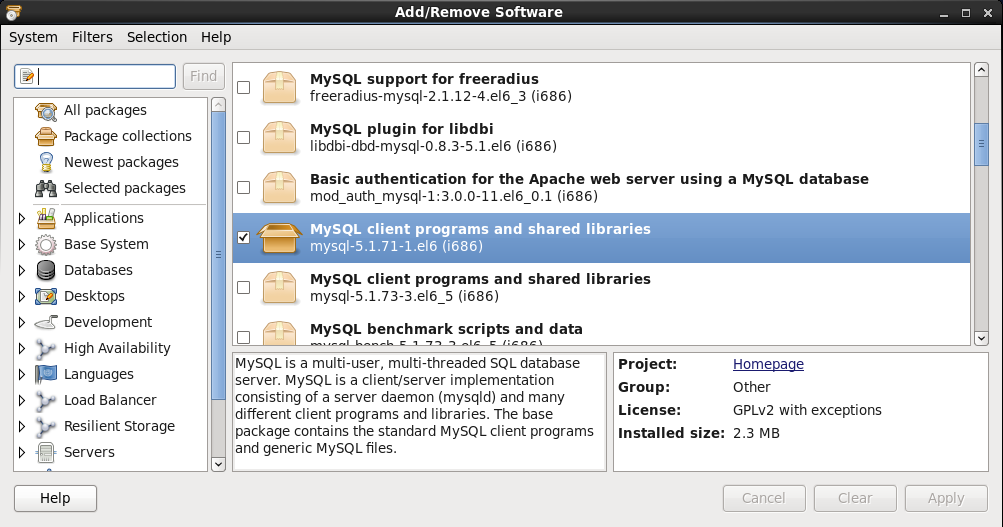
\includegraphics[scale=0.4]{Immagini/packagekit1.png}
  \label{fig:PackageKit}
  \caption{PackageKit front-end}
\end{figure}


Il tool da interfaccia grafica PackageKit, permette, attraverso una serie di menù intuitivi e guidati, di compiere tutte le operazioni relative alla ricerca, download, installazione, aggiornamento o rimozione dei pacchetti. 
PackageKit si basa su yum, ed è reperibile nel menu alla voce \menu{System > Administration > Add/Remove Software}.




\newpage

\section{Rete}

\subsection{Le Reti IP}

Con il concetto di rete, si intende l'insieme di canali fisici, protocolli ed implementazioni software che permettono agli elaboratori di poter comunicare attraverso delle opportune intefacce di rete.

Le tipologie di intefacce sono numerose, e, osservando anche quelle più affermate, si può notare quanto siano diversificate a livello fisico (es. Ethernet, ADSL, HSDPA/4G, Wireless...).

Ciò nonostante è possibile, attraverso opportune strumentazioni (gateway, router), e possibile far ``parlare'' gli elaboratori tra di loro, sfruttando dei protocolli comuni; senza nulla togliere  

\newpage


\end{document}

%
%\usepackage{subfigure}